% Generated by pysimcount.pfchilds -- do not edit; regenerate instead.
% figure: optimised-total-all-formulas -- Every formula, Nam Light optimised step, total gates vs n
% source: ../np-optimised-seeds/aggregate.json (seeds [1, 2, 3, 4, 5, 6, 7, 8, 9, 10]); run commits: e42ff29056ad9ea7fc7c9899fab334903e42e3e3
% metric=total kind=optimised merged (cz, simcount template)
% measured n: mean over seeds of the run's totals; bars min..max over seeds
% r from power-law fit to mean measured r (n = 5--10); r = ceil(a n^b); point=mean-r-fit; bars = min..max of per-seed fits
% per-step counts exactly affine in n (checked on n = [10, 13, 16])
% n > 16: optimised per-step count from linear fit (n = 10--16); circuit not built or verified
% shown: suzuki4, suzuki6, mo-q6, mo-q14, bm-q10, mo-o8-q21, morales-y8m10, morales-m8
% removed (see optimised-total-all-formulas-ranking.md): lie-trotter, suzuki2, suzuki8
% figure made at git_commit=e5d9ee696f892e28aced765585653760f8a427c4 git_dirty=False
% derived: optimised-total-all-formulas.tex restyled by pysimcount.figuniform: extrapolated points (r from power-law fit) drawn in their series' measured style, style-key legend entries removed; extrapolated n = [13, 20, 30, 50, 70, 100, 200, 300, 500]; source_sha256=9d045a840c2247ea94632fa5fb1e18e042599591ec6e676d39f9146be69c4bb6
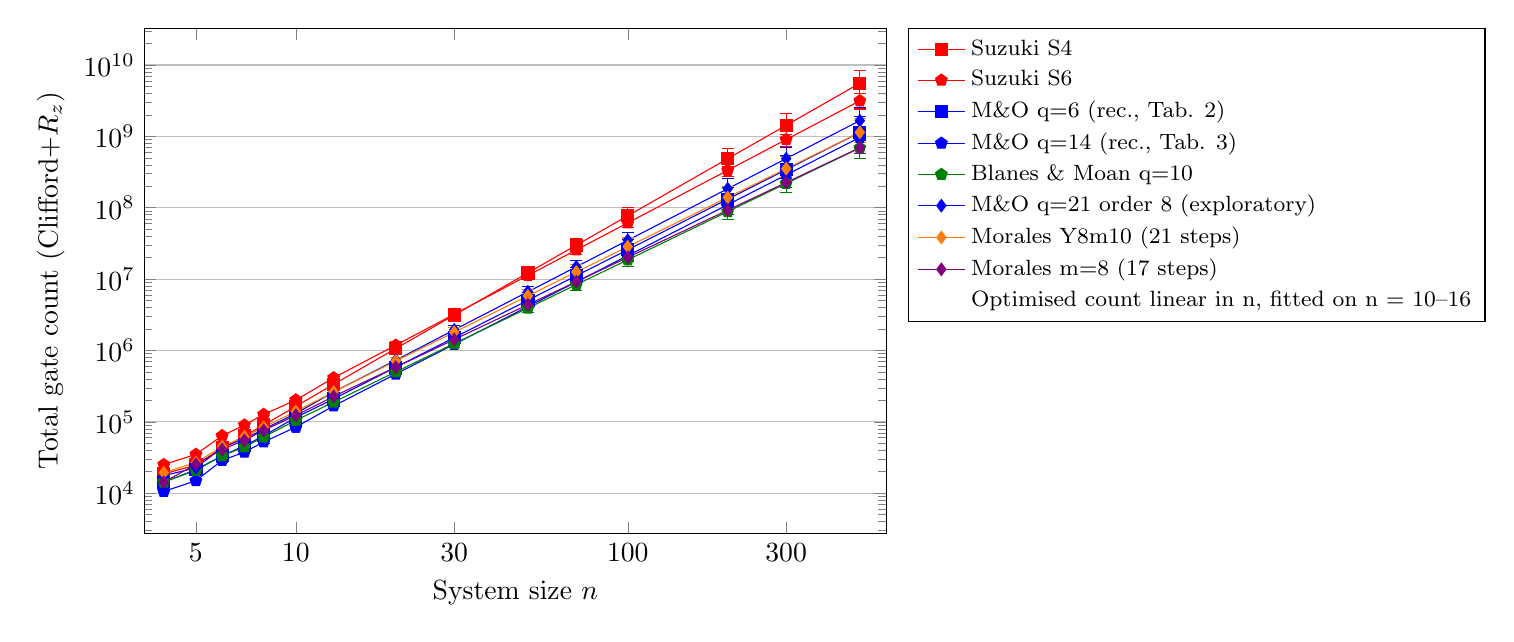
\begin{tikzpicture}
  \begin{loglogaxis}[
    width=11cm, height=8cm,
    xlabel={System size $n$},
    ylabel={Total gate count (Clifford+$R_z$)},
    xtick={5,10,30,100,300}, xticklabels={5,10,30,100,300},
    xmin=3.5, xmax=600,
    ymajorgrids=true,
    legend pos=outer north east,
    legend cell align=left,
    legend style={font=\footnotesize},
  ]
    % suzuki4: measured n, mean over seeds, bars min..max over seeds
    \addplot[red, solid, mark=square*, mark size=2.2pt, mark options={solid, fill=red}, error bars/.cd, y dir=both, y explicit, error bar style={solid}] coordinates {
      (4,18648) += (0,252) -= (0,168)
      (5,24824) += (0,856) -= (0,749)
      (6,43095) += (0,3055) -= (0,2145)
      (7,63189) += (0,4896) -= (0,4284)
      (8,90464) += (0,3696) -= (0,3344)
      (10,164946) += (0,12654) -= (0,6216)
    };
    \addlegendentry{Suzuki S4}
    % suzuki4: extrapolated, r = ceil(3.30875 n^1.65448), per step = 115 n + -40; bars min..max of per-seed fits
    \addplot[red, solid, mark=square*, mark size=2.2pt, mark options={solid, fill=red}, forget plot, error bars/.cd, y dir=both, y explicit, error bar style={solid}] coordinates {
      (10,164946)
      (13,336105) += (0,20370) -= (0,18915)
      (20,1.06446e+06) += (0,113000) -= (0,92660)
      (30,3.1372e+06) += (0,477400) -= (0,358050)
      (50,1.22251e+07) += (0,2.58663e+06) -= (0,1.81007e+06)
      (70,2.99254e+07) += (0,7.53741e+06) -= (0,5.08635e+06)
      (100,7.72404e+07) += (0,2.28856e+07) -= (0,1.48751e+07)
      (200,4.87142e+08) += (0,1.8857e+08) -= (0,1.14341e+08)
      (300,1.43002e+09) += (0,6.33685e+08) -= (0,3.69446e+08)
      (500,5.55179e+09) += (0,2.87024e+09) -= (0,1.59365e+09)
    };
    % suzuki6: measured n, mean over seeds, bars min..max over seeds
    \addplot[red, solid, mark=pentagon*, mark size=2.2pt, mark options={solid, fill=red}, error bars/.cd, y dir=both, y explicit, error bar style={solid}] coordinates {
      (4,25200) += (0,0) -= (0,0)
      (5,35042.5) += (0,2407.5) -= (0,267.5)
      (6,64025) += (0,4225) -= (0,2275)
      (7,90270) += (0,5355) -= (0,6120)
      (8,127160) += (0,4840) -= (0,3960)
      (10,202020) += (0,14430) -= (0,7770)
    };
    \addlegendentry{Suzuki S6}
    % suzuki6: extrapolated, r = ceil(1.3813 n^1.44491), per step = 575 n + -200; bars min..max of per-seed fits
    \addplot[red, solid, mark=pentagon*, mark size=2.2pt, mark options={solid, fill=red}, forget plot, error bars/.cd, y dir=both, y explicit, error bar style={solid}] coordinates {
      (10,202020)
      (13,414675) += (0,21825) -= (0,14550)
      (20,1.1865e+06) += (0,135600) -= (0,67800)
      (30,3.22245e+06) += (0,511500) -= (0,255750)
      (50,1.12487e+07) += (0,2.5124e+06) -= (0,1.1991e+06)
      (70,2.5672e+07) += (0,6.76845e+06) -= (0,3.24405e+06)
      (100,6.14256e+07) += (0,1.91382e+07) -= (0,8.9961e+06)
      (200,3.34986e+08) += (0,1.36382e+08) -= (0,6.16476e+07)
      (300,9.03369e+08) += (0,4.20584e+08) -= (0,1.85567e+08)
      (500,3.15082e+09) += (0,1.71231e+09) -= (0,7.29167e+08)
    };
    % mo-q6: measured n, mean over seeds, bars min..max over seeds
    \addplot[blue, solid, mark=square*, mark size=2.2pt, mark options={solid, fill=blue}, error bars/.cd, y dir=both, y explicit, error bar style={solid}] coordinates {
      (4,14263.2) += (0,856.8) -= (0,1663.2)
      (5,21442.8) += (0,1027.2) -= (0,2182.8)
      (6,33462) += (0,858) -= (0,1482)
      (7,46359) += (0,2295) -= (0,3213)
      (8,63782.4) += (0,5913.6) -= (0,3590.4)
      (10,115351) += (0,4528.8) -= (0,7459.2)
    };
    \addlegendentry{M\&O q=6 (rec., Tab. 2)}
    % mo-q6: extrapolated, r = ceil(3.76178 n^1.34927), per step = 138 n + -48; bars min..max of per-seed fits
    \addplot[blue, solid, mark=square*, mark size=2.2pt, mark options={solid, fill=blue}, forget plot, error bars/.cd, y dir=both, y explicit, error bar style={solid}] coordinates {
      (10,115351)
      (13,209520) += (0,19206) -= (0,10476)
      (20,583080) += (0,81360) -= (0,46104)
      (30,1.51813e+06) += (0,294624) -= (0,163680)
      (50,5.05678e+06) += (0,1.34984e+06) -= (0,705756)
      (70,1.11691e+07) += (0,3.5276e+06) -= (0,1.80706e+06)
      (100,2.58538e+07) += (0,9.57139e+06) -= (0,4.75819e+06)
      (200,1.31919e+08) += (0,6.36727e+07) -= (0,2.97011e+07)
      (300,3.42146e+08) += (0,1.89061e+08) -= (0,8.4937e+07)
      (500,1.13654e+09) += (0,7.39648e+08) -= (0,3.14214e+08)
    };
    % mo-q14: measured n, mean over seeds, bars min..max over seeds
    \addplot[blue, solid, mark=pentagon*, mark size=2.2pt, mark options={solid, fill=blue}, error bars/.cd, y dir=both, y explicit, error bar style={solid}] coordinates {
      (4,10584) += (0,0) -= (0,0)
      (5,14980) += (0,0) -= (0,0)
      (6,28938) += (0,182) -= (0,1638)
      (7,37699.2) += (0,856.8) -= (0,1285.2)
      (8,52236.8) += (0,1971.2) -= (0,2956.8)
      (10,84537.6) += (0,2486.4) -= (0,621.6)
    };
    \addlegendentry{M\&O q=14 (rec., Tab. 3)}
    % mo-q14: extrapolated, r = ceil(1.21616 n^1.36863), per step = 322 n + -112; bars min..max of per-seed fits
    \addplot[blue, solid, mark=pentagon*, mark size=2.2pt, mark options={solid, fill=blue}, forget plot, error bars/.cd, y dir=both, y explicit, error bar style={solid}] coordinates {
      (10,84537.6)
      (13,167034) += (0,8148) -= (0,4074)
      (20,468272) += (0,31640) -= (0,12656)
      (30,1.22214e+06) += (0,124124) -= (0,38192)
      (50,4.1249e+06) += (0,511616) -= (0,175868)
      (70,9.15062e+06) += (0,1.32325e+06) -= (0,426132)
      (100,2.13385e+07) += (0,3.52968e+06) -= (0,1.15517e+06)
      (200,1.10254e+08) += (0,2.30151e+07) -= (0,7.13597e+06)
      (300,2.88306e+08) += (0,6.72521e+07) -= (0,2.05519e+07)
      (500,9.66937e+08) += (0,2.5726e+08) -= (0,7.67436e+07)
    };
    % bm-q10: measured n, mean over seeds, bars min..max over seeds
    \addplot[green!50!black, solid, mark=pentagon*, mark size=2.2pt, mark options={solid, fill=green!50!black}, error bars/.cd, y dir=both, y explicit, error bar style={solid}] coordinates {
      (4,14364) += (0,756) -= (0,84)
      (5,20972) += (0,428) -= (0,642)
      (6,33410) += (0,390) -= (0,910)
      (7,44523) += (0,1377) -= (0,1683)
      (8,61248) += (0,3872) -= (0,3168)
      (10,105228) += (0,1332) -= (0,3108)
    };
    \addlegendentry{Blanes \& Moan q=10}
    % bm-q10: extrapolated, r = ceil(2.67799 n^1.24119), per step = 230 n + -80; bars min..max of per-seed fits
    \addplot[green!50!black, solid, mark=pentagon*, mark size=2.2pt, mark options={solid, fill=green!50!black}, forget plot, error bars/.cd, y dir=both, y explicit, error bar style={solid}] coordinates {
      (10,105228)
      (13,189150) += (0,8730) -= (0,8730)
      (20,501720) += (0,40680) -= (0,40680)
      (30,1.24806e+06) += (0,143220) -= (0,136400)
      (50,3.92848e+06) += (0,616680) -= (0,559580)
      (70,8.37846e+06) += (0,1.5219e+06) -= (0,1.39374e+06)
      (100,1.86569e+07) += (0,3.94224e+06) -= (0,3.52968e+06)
      (200,8.83042e+07) += (0,2.40621e+07) -= (0,2.05262e+07)
      (300,2.19166e+08) += (0,6.78862e+07) -= (0,5.62387e+07)
      (500,6.88945e+08) += (0,2.46388e+08) -= (0,1.97088e+08)
    };
    % mo-o8-q21: measured n, mean over seeds, bars min..max over seeds
    \addplot[blue, solid, mark=diamond*, mark size=2.2pt, mark options={solid, fill=blue}, error bars/.cd, y dir=both, y explicit, error bar style={solid}] coordinates {
      (4,17640) += (0,0) -= (0,0)
      (5,22694.7) += (0,2022.3) -= (0,224.7)
      (6,43680) += (0,2730) -= (0,2730)
      (7,58155.3) += (0,2891.7) -= (0,3534.3)
      (8,78724.8) += (0,2587.2) -= (0,4804.8)
      (10,131002) += (0,8857.8) -= (0,5128.2)
    };
    \addlegendentry{M\&O q=21 order 8 (exploratory)}
    % mo-o8-q21: extrapolated, r = ceil(1.17031 n^1.39675), per step = 483 n + -168; bars min..max of per-seed fits
    \addplot[blue, solid, mark=diamond*, mark size=2.2pt, mark options={solid, fill=blue}, forget plot, error bars/.cd, y dir=both, y explicit, error bar style={solid}] coordinates {
      (10,131002)
      (13,262773) += (0,12222) -= (0,12222)
      (20,730884) += (0,75936) -= (0,56952)
      (30,1.94779e+06) += (0,272118) -= (0,214830)
      (50,6.64301e+06) += (0,1.31901e+06) -= (0,959280)
      (70,1.49034e+07) += (0,3.53241e+06) -= (0,2.48951e+06)
      (100,3.50401e+07) += (0,9.96332e+06) -= (0,6.64222e+06)
      (200,1.84764e+08) += (0,6.96239e+07) -= (0,4.30087e+07)
      (300,4.8847e+08) += (0,2.12032e+08) -= (0,1.25338e+08)
      (500,1.66229e+09) += (0,8.46593e+08) -= (0,4.75183e+08)
    };
    % morales-y8m10: measured n, mean over seeds, bars min..max over seeds
    \addplot[orange, solid, mark=diamond*, mark size=2.2pt, mark options={solid, fill=orange}, error bars/.cd, y dir=both, y explicit, error bar style={solid}] coordinates {
      (4,19404) += (0,0) -= (0,0)
      (5,26964) += (0,0) -= (0,0)
      (6,45045) += (0,1365) -= (0,1365)
      (7,61689.6) += (0,2570.4) -= (0,642.6)
      (8,84268.8) += (0,4435.2) -= (0,2956.8)
      (10,139860) += (0,9324) -= (0,4662)
    };
    \addlegendentry{Morales Y8m10 (21 steps)}
    % morales-y8m10: extrapolated, r = ceil(1.56103 n^1.28936), per step = 483 n + -168; bars min..max of per-seed fits
    \addplot[orange, solid, mark=diamond*, mark size=2.2pt, mark options={solid, fill=orange}, forget plot, error bars/.cd, y dir=both, y explicit, error bar style={solid}] coordinates {
      (10,139860)
      (13,262773) += (0,18333) -= (0,12222)
      (20,711900) += (0,85428) -= (0,56952)
      (30,1.80457e+06) += (0,300762) -= (0,186186)
      (50,5.82763e+06) += (0,1.34299e+06) -= (0,815388)
      (70,1.25821e+07) += (0,3.46513e+06) -= (0,2.01852e+06)
      (100,2.84941e+07) += (0,9.19321e+06) -= (0,5.19826e+06)
      (200,1.39537e+08) += (0,5.85342e+07) -= (0,3.14368e+07)
      (300,3.53146e+08) += (0,1.69481e+08) -= (0,8.77076e+07)
      (500,1.13764e+09) += (0,6.36392e+08) -= (0,3.15421e+08)
    };
    % morales-m8: measured n, mean over seeds, bars min..max over seeds
    \addplot[violet, solid, mark=diamond*, mark size=2.2pt, mark options={solid, fill=violet}, error bars/.cd, y dir=both, y explicit, error bar style={solid}] coordinates {
      (4,14280) += (0,0) -= (0,0)
      (5,25466) += (0,0) -= (0,0)
      (6,41106) += (0,884) -= (0,1326)
      (7,55141.2) += (0,2080.8) -= (0,520.2)
      (8,75996.8) += (0,4787.2) -= (0,1196.8)
      (10,123032) += (0,5283.6) -= (0,2264.4)
    };
    \addlegendentry{Morales m=8 (17 steps)}
    % morales-m8: extrapolated, r = ceil(2.09405 n^1.19638), per step = 391 n + -136; bars min..max of per-seed fits
    \addplot[violet, solid, mark=diamond*, mark size=2.2pt, mark options={solid, fill=violet}, forget plot, error bars/.cd, y dir=both, y explicit, error bar style={solid}] coordinates {
      (10,123032)
      (13,227562) += (0,4947) -= (0,9894)
      (20,583984) += (0,38420) -= (0,30736)
      (30,1.42606e+06) += (0,127534) -= (0,92752)
      (50,4.38756e+06) += (0,563006) -= (0,368866)
      (70,9.20509e+06) += (0,1.41617e+06) -= (0,898722)
      (100,2.01834e+07) += (0,3.62365e+06) -= (0,2.25991e+06)
      (200,9.25839e+07) += (0,2.16237e+07) -= (0,1.27244e+07)
      (300,2.25658e+08) += (0,5.9988e+07) -= (0,3.42119e+07)
      (500,6.93347e+08) += (0,2.13142e+08) -= (0,1.18e+08)
    };
    \addlegendimage{empty legend}
    \addlegendentry{Optimised count linear in n, fitted on n = 10--16}
  \end{loglogaxis}
\end{tikzpicture}
